\section{Data structure}
The data is stored in a matrix of so-called \emph{hits}, which is a single count/detection registered on a detector. The acquisition software can group these hits, because they are expected to be related to each other; this is called an \emph{event}. The start of an event is usually defined by a trigger (which could be a hit on one of the detectors), the duration of an event can be defined by a timeframe from the event start.

\begin{figure}[h]
   \centering
    \centerline{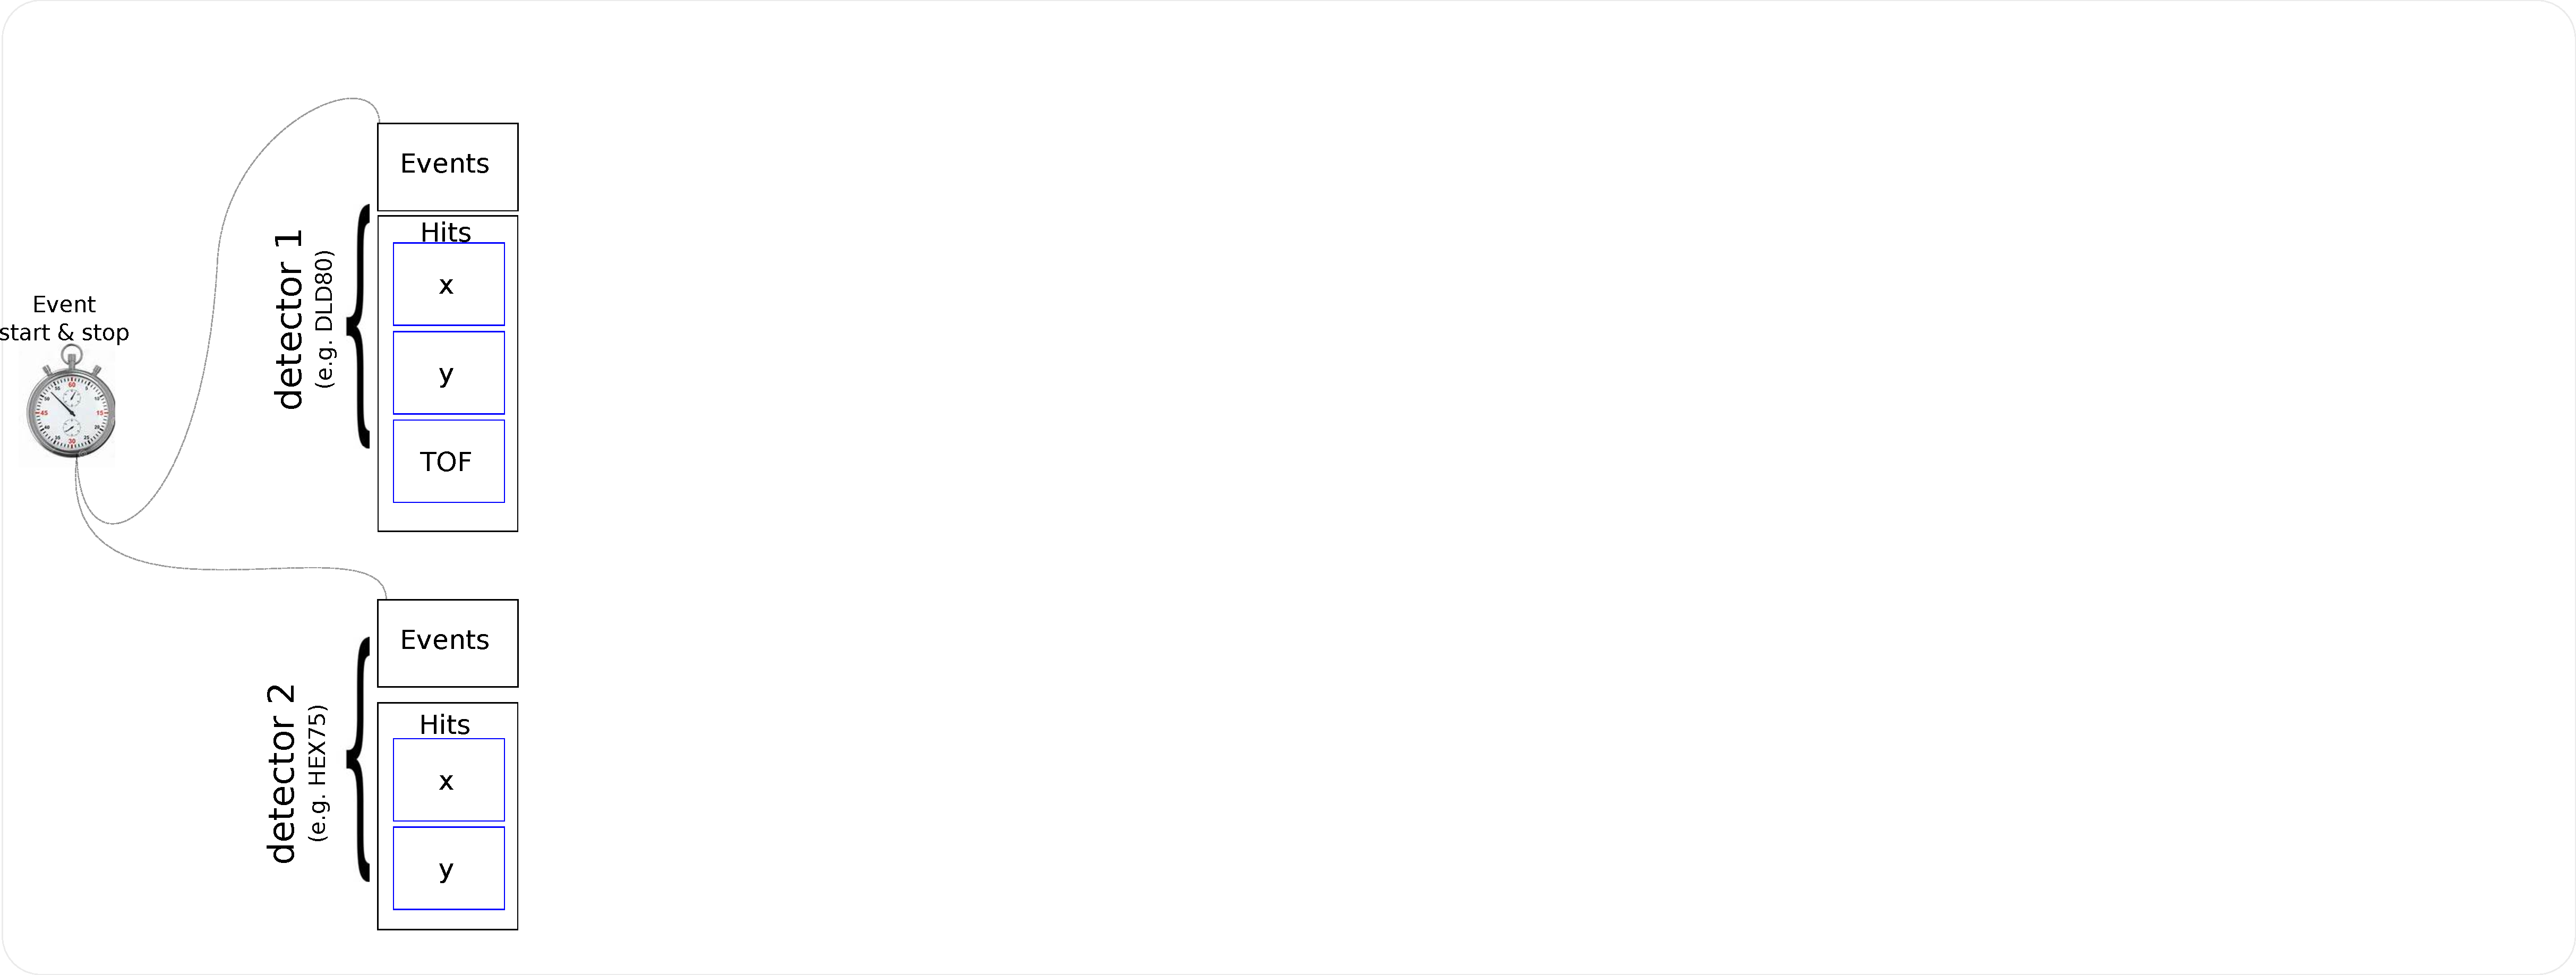
\includegraphics[width=1\textwidth]{Graphics/synchronization.pdf}}
\caption{The synchronization of events by a common 'clock'.}
\label{event_synchronization}
\end{figure}

For example, an event from an experiment on \ce{H_2O} is the registration of two hits on the ion detector: one from H$^+$ and after that one from OH$^+$, and the registration of two hits on the electron detector. Note that the number of hits is generally different for different detectors.
\\
The matrix of hits only contains the data that is given along with every hit (for example X, Y and T), but it does not show to which event the hit belonged. The grouping of events is done in another matrix, that contains the \emph{event pointers}. The list of event pointers contains the index of the \emph{first hit} of that event. 
This structure is chosen, because it can easily be extended when the measurement uses multiple detectors.
Important to notice is that the events from different detectors are synchronized; every event start is measured at the same instant in time. 

A schematic of the data structure is shown in Figure \ref{Data_structure_schematic_intro}.

\begin{figure}[h]
   \centering
    \centerline{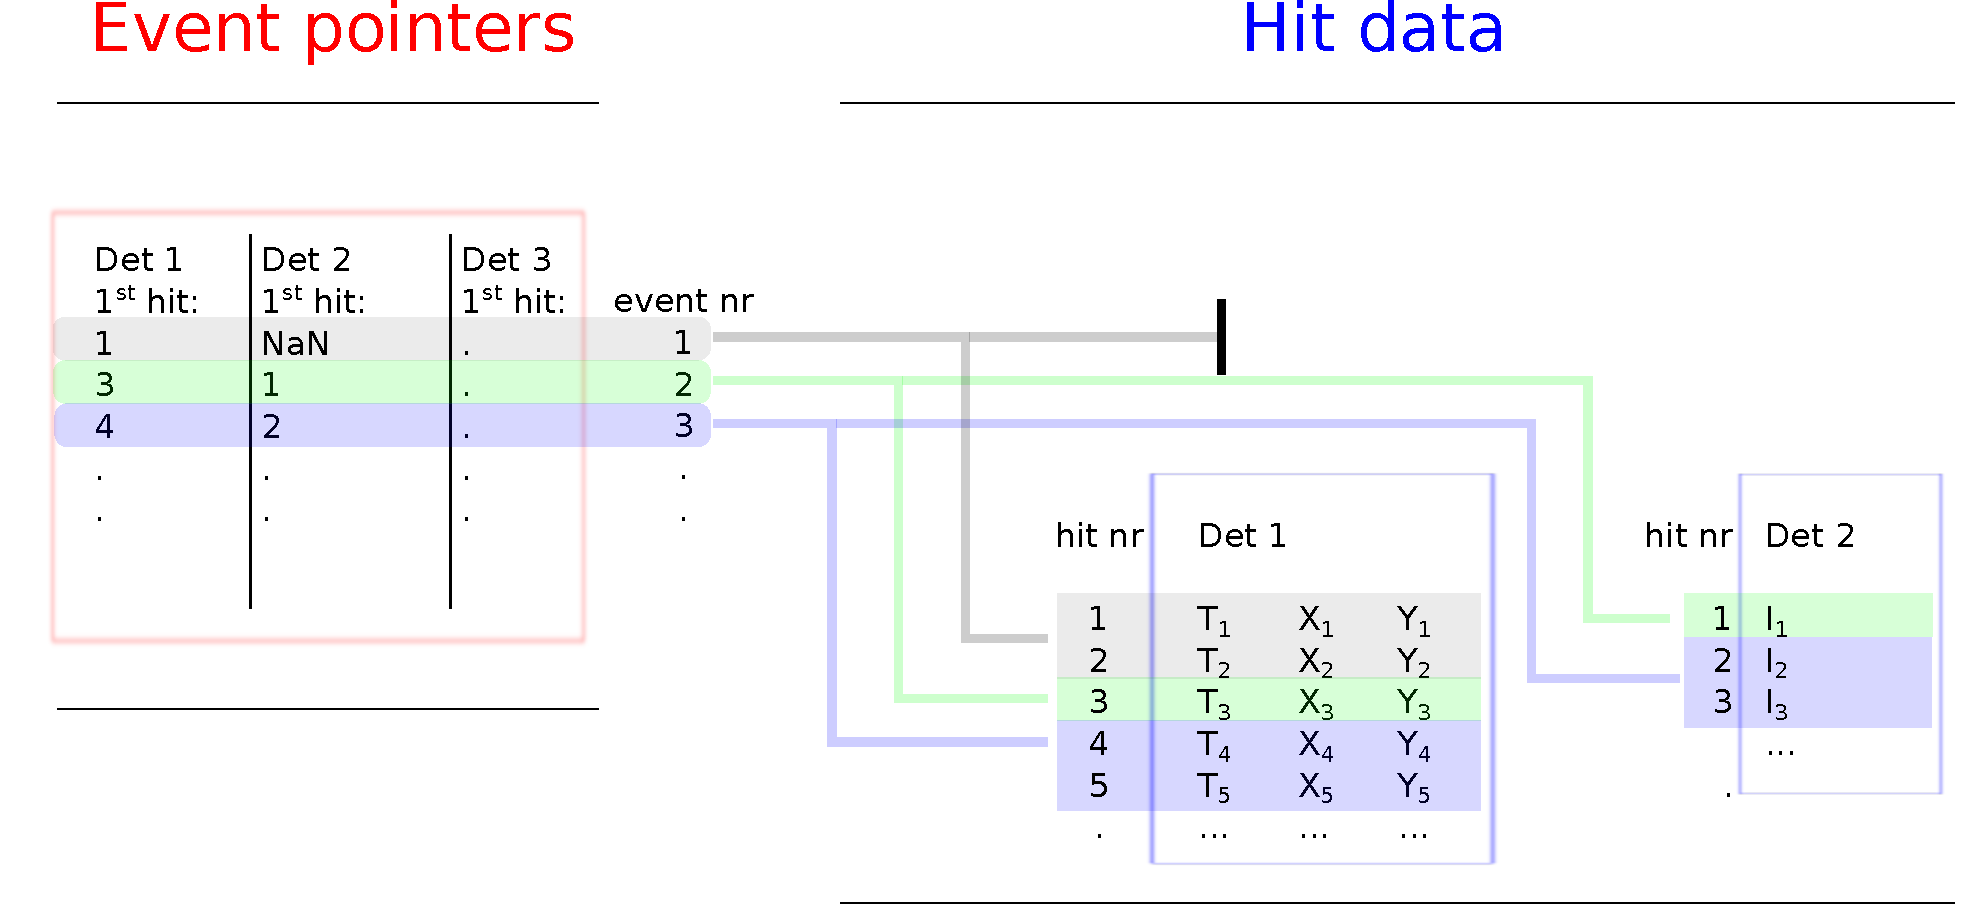
\includegraphics[width=0.9\textwidth]{Graphics/data_structure_schematic.pdf}}
\caption{Schematic of the data structure used in the software. The `event pointers' array on the left stores the indeces of the first hit of the event, for each different detector used (in this case two detectors). On the right, the hit arrays are drawn, with the hits coming from these detectors. Note that each detector can give another number of hits, and a different number of signals (e.g. X, Y, T, Intensity). In this example, there are no hits recorded on detector 2 during event 1, which is denoted by `NaN' (not-a-number).}
\label{Data_structure_schematic_intro}
\end{figure}

The naming in the .MAT file is such, that all data is the subfields `e' (for events) and `h' (for hits). An example of a set of raw files is given below:

\lstset{language=MATLAB}
\begin{lstlisting}
exp1.e.raw ;% 	event pointers. size: [nof_events, nof_det]. 
exp1.h.det1.raw ;% detector 1 hits [nof_hits(1), nof_signals(1)]
exp1.h.det1.raw_sn ;% cell with signal names from det 1 [1, nof_signals(1)]
exp1.h.det2.raw ;% detector 2 hits [nof_hits(2), nof_signals(2)]
exp1.h.det2.raw_sn ;% cell with signal names from det 2 [1, nof_signals(2)]
\end{lstlisting}

The name `exp1' can be changed, so that several different experiments can be opened at the same time.
